\documentclass[a4paper, titlepage,11pt]{article}
\usepackage{fontspec}
\usepackage{polyglossia}
\setdefaultlanguage{english}
\usepackage{indentfirst}
\usepackage{graphicx}
\usepackage{float}
\usepackage{microtype}
\usepackage{standalone}
\usepackage[sorting=none,backend=biber]{biblatex}
\usepackage[inline]{enumitem}
\usepackage{booktabs}
\usepackage[font=small,justification=centering]{caption}
\usepackage{subcaption}
\usepackage{csquotes}
\usepackage{amsmath}
\usepackage{amsfonts}
\usepackage{mathrsfs}
\usepackage{tikz}
\usepackage{tikz-cd}
\usepackage{quiver}
\usepackage{algorithm}
\usepackage{algpseudocode}
% \usepackage{changes}
\usepackage[hidelinks]{hyperref}
\usepackage{xcolor}
\usepackage[ampersand]{easylist}
\usepackage{placeins}
\usepackage{scalefnt}

\usetikzlibrary{positioning,shapes.misc, calc, graphs, graphdrawing}
\usegdlibrary{trees}
\brokenpenalty=1000
\clubpenalty=1000
\widowpenalty=1000
% \definechangesauthor[name={AP}, color=blue]{ap}

% \DeclareMathOperator{\sigm}{sigm}
% \DeclareMathOperator{\patches}{patches}
% \DeclareMathOperator{\CrsEnt}{\mathcal{L}_{CE}}
% \DeclareMathOperator{\Sep}{\mathcal{L}_{Sep}}
% \DeclareMathOperator{\Clst}{\mathcal{L}_{Clst}}
% \DeclareMathOperator{\sigmaop}{\sigma}

\newcommand{\change}[1]{#1}


\title{Fractal Wavelet Image Compression}
\author{}
\date{\today}

\addbibresource{main.bib}
\makeatletter

\begin{document}
    \newcommand{\horrule}[1]{\rule{\linewidth}{#1}} 
\newcommand\doubleRule{\toprule\toprule}
\newcommand\doublerule{\toprule\specialrule{\heavyrulewidth}{\doublerulesep}{0.4em}}
\newcommand{\ra}[1]{\renewcommand{\arraystretch}{#1}}
\renewcommand*{\hbar}{\mathalpha{\usebox{\myhbar}}}
\begin{titlepage}
\centering
%\vspace*{1cm}
\Large
\textsc{Jagiellonian University \\ Institute of Computer Science and Computational Mathematics \\ Faculty of Mathematics and Computer Science} \\ \vspace*{1\baselineskip}


\includegraphics[width=0.25\textwidth,height=0.25\textheight,keepaspectratio]{uj_logo.jpg}

\horrule{0.5pt} \\[0.4cm] % Thin top horizontal rule
\Huge  Fractal Wavelet Image Compression \\ 
\horrule{2pt} \\[0.5cm] % Thick bottom horizontal rule

\Large{Master thesis \\ \textit{submitted by}}
\vspace*{1\baselineskip}

\LARGE \textbf{Paweł Gmerek} \\
\vspace*{1\baselineskip}

\Large{\textit{supervised by:} \\dr Jarosław Duda\\}
    
\vspace*{2\baselineskip}
\Large{Kraków, 2025}

\end{titlepage}

    \empty
    \begin{abstract}

Image compression algorithms are ubiquitous in modern computer systems. Lossy codecs allow
to save exabytes of memory worldwide and they do that by eliminating redundant visual data
in images they compress. For both DCT and wavelet apporaches they divide an image into blocks 
of fixed or variadic size and then for each block perform quantization and entropy encoding. 
With harsher compression approaches there are visible compression defects called block artifacts.
I will attempt to approach this common limitation with a novel FRIF compression algorithm that introduces
more irregular boundary by replacing blocks with complex-based fractals to cover the image.
Such covering also benefits from hexagonal nature of presented fractals, giving six immiediate neighbours for 
statistical modeling and prediction.

\bigskip
\noindent \textbf{Keywords:}
\begin{itemize*}[label={},itemjoin={{ $\cdot$}}]
    \item Image compression
    \item Wavelet transform
    \item Complex-based numeral systems
    \item ANS
    \item Statistical modeling
\end{itemize*}
\end{abstract}


    
    \microtypesetup{protrusion=false}
    \tableofcontents
    \microtypesetup{protrusion=true}
    %\listoffigures
    \clearpage
    
    \section{Introduction}


As digital images began to be stored and transmitted over networks, the need to reduce their size became essential.
In natural photographic images, neighboring pixels tend to be highly correlated; for example,
a pixel in a sky region usually has color values similar to its surrounding pixels.
Compression algorithms exploit this spatial redundancy to efficiently reduce image data without significant loss of quality.
Codecs start the compression scheme by transforming input image into an intermediate representation, that has better statistical parameters for
entropy encoding. Historically most popular such transformations were DCT (Discrete Cosine Transform) and DWT
(Discrete Wavelet Transform), both of which transform the input space by dividing it into a grid of blocks and then
performing further operations within each one. Such transformed image still contains a lot of information that is missed
by human vision. Alterations in high-frequency components are generally less perceptible to the visual cortex. To further diminish the size of the transformed representation, quantization is employed in lossy codecs to effectively discard those values that remain undetected.
This approach proved to achieve best results in modern codecs, but with harsher
quantization in lossy compression block boundaries are much more visible. 
Lossless codecs often used block lattices for context modelling and better prediction of residuals. Each block is directly adjacent 
to 4 different blocks and can infer its values from those neighbors. In JPEG-LS \cite{weinberger1996LOCO} authors proposed a predictor
LOCO-I that assigns each element to one of 365 contexts based on the already decoded neighboring values adjusting 
the distributions of encoded elements. Such grouping enables codec to use different instances of entropy coder for 
different probability distributions observed within each context.

\begin{figure}[ht]
    \centering
    {
    \setlength{\fboxsep}{0pt}
    \setlength{\fboxrule}{1pt}
    \fbox{
\includegraphics[scale=1.5]{figures/introduction/rect_grid.jpg}}
    }
    \caption{Plane decomposition into rectangular grid}
    
\end{figure}

Building ahead of these ideas and problems I will present a novel image compression codec \textbf{FRIF} (\textbf{FR}actal \textbf{I}mage \textbf{F}ormat)
which presents a new idea of fractal lattice decomposition of an image with discrete wavelet transform applied to each fractal region. Such grid
has a certain amount of interesting properties that could be leveraged in mentioned image compression methods:
\begin{itemize}
    \item Complex numeral systems fractals have a highly irregular boundary
    \item Since each fractal has 6 immediate neighbors, we get an hexagonal grid which allow inferring contexts and 
        predictions from a larger set
    \item Self-similarity relation of each fractal can benefit from wavelet transform decomposition
\end{itemize}
\begin{figure}[ht]
    \centering
    {
        \setlength{\fboxsep}{0pt}
        \setlength{\fboxrule}{1pt}
        \fbox{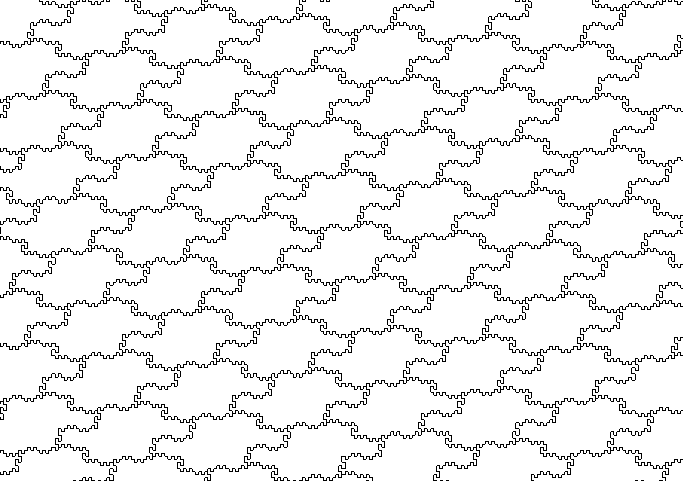
\includegraphics[scale=1.5]{figures/introduction/fractal_grid.png}}
    }
    \caption{Plane decomposition into tame-twindragon fractals}

\end{figure}
Along with the thesis implementation of the codec will be presented with comparisons to the existing lossless and lossy
popular approaches.
Experiments will be carried out over 3 datasets: kodak \cite{kodakdataset}, CID22 \cite{CID22} and JSI31 \cite{J31}
to collect average bits per pixel value corresponding to the compression ratio and SSIM2 metric to assess image quality after quantization.

Aim of this thesis is not to beat current sophisticated compression models with FRIF, but 
to measure performance of a quite different approach. The remainder of this thesis is organized as follows:
Section 2 presents the preliminaries required to state the compression algorithm, including complex-based numeral systems, wavelet transform and chosen entropy encoder.
Section 3 fully describes the FRIF compression algorithm, including all stages of compression and chosen image format to store compressed images on disk, giving the official
and full specification of this compression scheme. 
Section 4 showcases experiments taken to measure performance of codec, including metrics like bits per pixel or the quality of compressed image on lossy compression. 
Finally, section 5 reviews the codec and states the conclusion of this novel and unique approach.













    \newpage
\section{Preliminaries}

\subsection{Complex based numeral systems}

\subsection{Discrete Haar wavelet transform}

\subsection{ANS entropy coding}

\subsection{Color transform}

    \newpage
\section{Compression method}

\subsection{Algorithm overview}

\subsection{Construction of fractal grid}

\subsection{Choice of wavelet}

\subsection{Prediction}

\subsection{Context modeling}

\subsection{Image format}


    \newpage
\section{Experiments}

\subsection{SSIM2 metric}

\subsection{J31 dataset}

\subsection{kodak dataset}

    \section{Summary}

Proposed compression algorithm shows promise in the lossless benchmarks, as on kodak dataset FRIF achieved overall better
compression rates than ubiquitous PNG format. Novel context modeling and prediction greatly enhanced the ability of the compressor to find spatial redundancies
and lower the amount of bits required to signal one pixel. This advantage quickly diminishes versus JPEG2000, a similar wavelet compressor, that
tacross all lossless benchmarks performed better. 
For lossy mode experiments showed that proposed quantization pattern produces pixelated versions of the original image, damaging the quality observed
via SSIM2 metric.

\subsection{Room for improvement}
There is a noticable room for improvement for presented codec and areas worth exploring to enhance both lossless and lossy compression ratios. 
One of them can be the choice of used wavelet in DWT, as Haar wavelet is the simplest wavelet that fitted the recursive tame-twindragon fractal nature. 
A wavelet more suited for image compression could benefit lossless mode, bringing FRIF closer to JPEG2000 performance.
The quantization scheme could potentially be enhanced by an approach similar to JPEGXL Modular mode with a tendency term, that limits the pixelation of dead-zoned
parameters. For a small compression ratio boost FRIF with better width prediction for context modelling could abandon saving \texttt{off\_distribution\_values} array as the image header.

\subsection{Closing remarks}
This thesis presented FRIF, a new image compression codec based on tame-twindragon fractal grid decomposition and discrete wavelet transform
with novel context modeling scheme. Although the lossy encoding mode requires additional refinement, FRIF gives a decent backbone of a codec that
can losslessly compress images with on-pair performance to PNG. Proposed solutions in grid selection, context modeling and prediction
with improvements mentioned in the thesis could yield even better results for both lossy and lossless compression, leaving space for further research. 
Presented compression scheme and implementation details can be found on an open-source repository hosted on GitHub under following URL: \url{https://github.com/pagmerek/frave}

   
    % \printbibliography[heading=bibintoc]
\end{document}
